% Options for packages loaded elsewhere
\PassOptionsToPackage{unicode}{hyperref}
\PassOptionsToPackage{hyphens}{url}
%
\documentclass[
  a4paper,
]{article}
\usepackage{amsmath,amssymb}
\usepackage{iftex}
\ifPDFTeX
  \usepackage[T1]{fontenc}
  \usepackage[utf8]{inputenc}
  \usepackage{textcomp} % provide euro and other symbols
\else % if luatex or xetex
  \usepackage{unicode-math} % this also loads fontspec
  \defaultfontfeatures{Scale=MatchLowercase}
  \defaultfontfeatures[\rmfamily]{Ligatures=TeX,Scale=1}
\fi
\usepackage{lmodern}
\ifPDFTeX\else
  % xetex/luatex font selection
\fi
% Use upquote if available, for straight quotes in verbatim environments
\IfFileExists{upquote.sty}{\usepackage{upquote}}{}
\IfFileExists{microtype.sty}{% use microtype if available
  \usepackage[]{microtype}
  \UseMicrotypeSet[protrusion]{basicmath} % disable protrusion for tt fonts
}{}
\makeatletter
\@ifundefined{KOMAClassName}{% if non-KOMA class
  \IfFileExists{parskip.sty}{%
    \usepackage{parskip}
  }{% else
    \setlength{\parindent}{0pt}
    \setlength{\parskip}{6pt plus 2pt minus 1pt}}
}{% if KOMA class
  \KOMAoptions{parskip=half}}
\makeatother
\usepackage{xcolor}
\usepackage[margin=1in]{geometry}
\usepackage{graphicx}
\makeatletter
\def\maxwidth{\ifdim\Gin@nat@width>\linewidth\linewidth\else\Gin@nat@width\fi}
\def\maxheight{\ifdim\Gin@nat@height>\textheight\textheight\else\Gin@nat@height\fi}
\makeatother
% Scale images if necessary, so that they will not overflow the page
% margins by default, and it is still possible to overwrite the defaults
% using explicit options in \includegraphics[width, height, ...]{}
\setkeys{Gin}{width=\maxwidth,height=\maxheight,keepaspectratio}
% Set default figure placement to htbp
\makeatletter
\def\fps@figure{htbp}
\makeatother
\setlength{\emergencystretch}{3em} % prevent overfull lines
\providecommand{\tightlist}{%
  \setlength{\itemsep}{0pt}\setlength{\parskip}{0pt}}
\setcounter{secnumdepth}{-\maxdimen} % remove section numbering
% definitions for citeproc citations
\NewDocumentCommand\citeproctext{}{}
\NewDocumentCommand\citeproc{mm}{%
  \begingroup\def\citeproctext{#2}\cite{#1}\endgroup}
\makeatletter
 % allow citations to break across lines
 \let\@cite@ofmt\@firstofone
 % avoid brackets around text for \cite:
 \def\@biblabel#1{}
 \def\@cite#1#2{{#1\if@tempswa , #2\fi}}
\makeatother
\newlength{\cslhangindent}
\setlength{\cslhangindent}{1.5em}
\newlength{\csllabelwidth}
\setlength{\csllabelwidth}{3em}
\newenvironment{CSLReferences}[2] % #1 hanging-indent, #2 entry-spacing
 {\begin{list}{}{%
  \setlength{\itemindent}{0pt}
  \setlength{\leftmargin}{0pt}
  \setlength{\parsep}{0pt}
  % turn on hanging indent if param 1 is 1
  \ifodd #1
   \setlength{\leftmargin}{\cslhangindent}
   \setlength{\itemindent}{-1\cslhangindent}
  \fi
  % set entry spacing
  \setlength{\itemsep}{#2\baselineskip}}}
 {\end{list}}
\usepackage{calc}
\newcommand{\CSLBlock}[1]{\hfill\break\parbox[t]{\linewidth}{\strut\ignorespaces#1\strut}}
\newcommand{\CSLLeftMargin}[1]{\parbox[t]{\csllabelwidth}{\strut#1\strut}}
\newcommand{\CSLRightInline}[1]{\parbox[t]{\linewidth - \csllabelwidth}{\strut#1\strut}}
\newcommand{\CSLIndent}[1]{\hspace{\cslhangindent}#1}
\usepackage{amsmath}
\usepackage{booktabs}
\DeclareMathOperator*{\argmax}{argmax}
\DeclareMathOperator*{\argmin}{argmin}
\DeclareMathOperator{\sgn}{sgn}
\ifLuaTeX
  \usepackage{selnolig}  % disable illegal ligatures
\fi
\usepackage{bookmark}
\IfFileExists{xurl.sty}{\usepackage{xurl}}{} % add URL line breaks if available
\urlstyle{same}
\hypersetup{
  pdftitle={Location and Scale-Invariant Power Transformations for Transforming Data to Normality},
  pdfauthor={Alex Zwanenburg, Steffen Löck},
  hidelinks,
  pdfcreator={LaTeX via pandoc}}

\title{Location and Scale-Invariant Power Transformations for
Transforming Data to Normality}
\author{Alex Zwanenburg, Steffen Löck}
\date{2024-10-17}

\begin{document}
\maketitle

\section{Abstract}\label{abstract}

To-do

\section{Introduction}\label{introduction}

Many statistical and some machine learning methods assume normality of
the underlying data, e.g.~analysis of variance and linear discriminant
analysis. However, numerical features in datasets may strongly deviate
from normal distributions, e.g.~by being skewed. Power transformations
aim to stabilise variance and improve normality of such features
(Bartlett 1947; John W. Tukey 1957). The two most commonly used
transformations are that of Box and Cox (1964) and Yeo and Johnson
(2000). The Box-Cox transformation of a feature value \(x_i\) of feature
\(\mathbf{X}=\left\{x_1, x_2, \ldots, x_n \right\}\) under the
transformation parameter \(\lambda\) is defined as:

\begin{equation}
\label{eqn:box-cox-original}
\phi_{\text{BC}}^\lambda (x_i) = 
\begin{cases}
\left(x_i^\lambda - 1 \right) / \lambda & \text{if } \lambda \neq 0\\
\log(x_i) & \text{if } \lambda = 0
\end{cases}
\end{equation}

One limitation of the Box-Cox transformation is that it is only defined
for \(x_i > 0\). In contrast, the Yeo-Johnson transformation under the
transformation parameter \(\lambda\) is defined for any
\(x_i \in \mathbb{R}\):

\begin{equation}
\label{eqn:yeo-johnson-original}
\phi_{\text{YJ}}^\lambda (x_i) = 
\begin{cases}
\left( \left( 1 + x_i \right)^\lambda - 1\right) / \lambda & \text{if } \lambda \neq 0 \text{ and } x_i \geq 0\\
\log(1 + x_i) & \text{if } \lambda = 0 \text{ and } x_i \geq 0\\
-\left( \left( 1 - x_i\right)^{2 - \lambda} - 1 \right) / \left(2 - \lambda \right) & \text{if } \lambda \neq 2 \text{ and } x_i < 0\\
-\log(1 - x_i) & \text{if } \lambda = 2 \text{ and } x_i < 0
\end{cases}
\end{equation}

The \(\lambda\)-parameter is typically optimised using maximum
likelihood estimation under the assumption that the transformed feature
is normally distributed. As noted by Raymaekers and Rousseeuw, this
approach is sensitive to outliers, and robust versions of Box-Cox and
Yeo-Johnson transformations were devised (Raymaekers and Rousseeuw
2024).

Applying a power transformation does not guarantee that transformed
features are normally distributed. Depending on location and scale of a
feature and the presence of outliers, power transformations may decrease
normality, as shown in Figure \ref{fig:decreased-normality}. If
normality of the transformed feature is not checked, e.g.~in automated
power transformation in machine learning workflows, several issues may
arise. For example, statistical tests such as ANOVA may produce
incorrect results due to violation of the normality assumption.
Likewise, machine learning methods that assume normality of input
features may suffer a decrease in performance. Moreover, large negative
or positive \(\lambda\)-parameters may lead to numeric issues in any
subsequent computations.

Statistical tests for normality, such as the Shapiro-Wilk test (Shapiro
and Wilk 1965), could be automatically applied to transformed features.
However, given sufficiently large sample sizes such tests can detect
trivial deviations from normality, and may lead to rejection of
sufficiently good power transformations.

\begin{figure}

{\centering 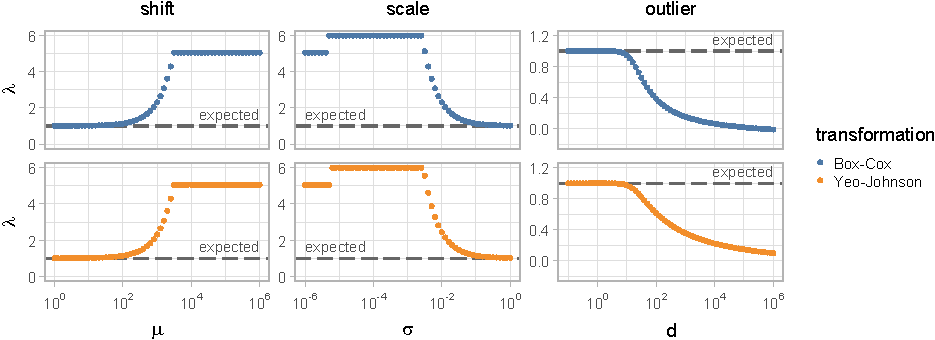
\includegraphics{manuscript_files/figure-latex/decreased-normality-1} 

}

\caption{Effect of location, scale and outliers on estimation of the Box-Cox and Yeo-Johnson transformation parameter $\lambda$. $10000$ samples were drawn from a normal distribution: $\mathcal{N}(\mu, 1)$ for the shift dataset, $\mathcal{N}(10, \sigma)$ for the scale dataset and $\mathcal{N}(0, 1)$ for the outlier dataset. Additionally, an outlier with value $d$ was added to the outlier dataset. Since samples are drawn from a normal distribution, a transformation parameter of $\lambda = 1$ is expected. However, a large shift in location, a scale that is small compared to the location, or presence of large outliers lead to incorrectly estimated transformation parameter values.}\label{fig:decreased-normality}
\end{figure}

To address these issues, we make the following contributions:

\begin{itemize}
\item
  We devise location- and scale-invariant versions of the Box-Cox and
  Yeo-Johnson transformation, including versions robust to outliers.
\item
  We derive the maximum likelihood criterion for location- and
  scale-invariant Box-Cox and Yeo-Johnson transformations to allow for
  optimising transformation parameters.
\item
  We define an empirical central normality test for detecting cases
  where power transformations fail to yield an approximately normally
  distributed transformed feature.
\item
  We assess the effect of power transformations on the performance of
  machine learning models.
\end{itemize}

\section{Theory}\label{theory}

In this section, we will first introduce location- and scale-invariant
versions of the Box-Cox and Yeo-Johnson transformations. Subsequently,
we define weighted location- and scale-invariant transformations and
weighting methods for robust transformations. We then define the
quantile function for asymmetric generalised normal distributions to
enable random sampling. Finally, we define the overall framework for the
empirical central normality test.

\subsection{Location- and scale-invariant power
transformation}\label{location--and-scale-invariant-power-transformation}

Box-Cox and Yeo-Johnson transformations are modified by introducing
shift parameter \(x_0\) and scale parameter \(s\) into equations
\ref{eqn:box-cox-original} and \ref{eqn:yeo-johnson-original}. The
location- and scale-invariant Box-Cox transformation of a feature value
\(x_i\) of feature \(\mathbf{X}\) under transformation parameter
\(\lambda\), shift parameter \(x_0\) and scale parameter \(s\) is then:

\begin{equation}
\label{eqn:box-cox-invariant}
\phi_{\text{BC}}^{\lambda, x_0, s} (x_i) = 
\begin{cases}
\left( \left(\frac{x_i - x_0}{s} \right)^\lambda - 1 \right) / \lambda & \text{if } \lambda \neq 0\\
\log\left[\frac{x_i - x_0}{s}\right] & \text{if } \lambda = 0
\end{cases}
\end{equation}

where \(x_i - x_0 > 0\). Likewise, the location- and scale-invariant
Yeo-Johnson transformation of a feature value \(x_i\) under
transformation parameter \(\lambda\), shift parameter \(x_0\) and scale
parameter \(s\) is:

\begin{equation}
\label{eqn:yeo-johnson-invariant}
\phi_{\text{YJ}}^{\lambda, x_0, s} (x_i) = 
\begin{cases}
\left( \left( 1 + \frac{x_i - x_0}{s}\right)^\lambda - 1\right) / \lambda & \text{if } \lambda \neq 0 \text{ and } x_i - x_0 \geq 0\\
\log\left[1 + \frac{x_i - x_0}{s}\right] & \text{if } \lambda = 0 \text{ and } x_i - x_0 \geq 0\\
-\left( \left( 1 - \frac{x_i - x_0}{s}\right)^{2 - \lambda} - 1 \right) / \left(2 - \lambda \right) & \text{if } \lambda \neq 2 \text{ and } x_i - x_0 < 0\\
-\log\left[1 - \frac{x_i - x_0}{s}\right] & \text{if } \lambda = 2 \text{ and } x_i - x_0 < 0
\end{cases}
\end{equation}

For both invariant transformations, \(\lambda\), \(x_0\) and \(s\)
parameters can be obtained by maximising the log-likelihood function,
i.e.~using maximum likelihood estimation (MLE). A full derivation of the
log-likelihood function for both transformations is shown in Appendix A.
The location- and scale-invariant Box-Cox log-likelihood function is:

\begin{equation}
\label{eqn:box-cox-invariant-log-likelihood}
\begin{split}
\mathcal{l}_{\text{BC}}^{\lambda, x_0, s} = & -\frac{n}{2} \log \left[2 \pi \sigma^2 \right] -\frac{1}{2 \sigma^2} \sum_{i=1}^n \left( \phi_{BC}^{\lambda, x_0, s}(x_i) - \mu \right)^2 \\
& -n \lambda \log s + \left( \lambda - 1 \right) \sum_{i=1}^n \log \left[ x_i - x_0 \right]
\end{split}
\end{equation}

subject to \(x_i - x_0 > 0\). \(\mu\) and \(\sigma^2\) are the mean and
variance of the Box-Cox transformed feature
\(\phi_{\text{BC}}^{\lambda, x_0, s} (\mathbf{X})\), respectively.
Similarly, the location- and scale-invariant Yeo-Johnson log-likelihood
function is:

\begin{equation}
\label{eqn:yeo-johnson-invariant-log-likelihood}
\begin{split}
\mathcal{l}_{\text{YJ}}^{\lambda, x_0, s} = & -\frac{n}{2} \log\left[2 \pi \sigma^2\right] -\frac{1}{2 \sigma^2} \sum_{i=1}^n \left( \phi_{YJ}^{\lambda, x_0, s}(x_i) - \mu \right)^2 \\
& - n \log s + (\lambda - 1) \sum_{i=1}^n \sgn(x_i - x_0) \log \left[1 + \frac{|x_i - x_0|}{s} \right]
\end{split}
\end{equation}

where \(\mu\) and \(\sigma^2\) are the mean and variance of the
Yeo-Johnson transformed feature
\(\phi_{\text{YJ}}^{\lambda, x_0, s} (\mathbf{X})\), respectively.

\subsection{Robust location- and scale-invariant power
transformations}\label{robust-location--and-scale-invariant-power-transformations}

Real-world data may contain outliers, to which maximum likelihood
estimation can be sensitive. Their presence may lead to poor
transformations to normality, as shown in Figure
\ref{fig:decreased-normality}. As indicated by Raymaekers and Rousseeuw
(2024), the general aim of power transformations should be to transform
non-outlier data to normality, i.e.~achieve \emph{central normality}. To
achieve this, they devised an iterative procedure to find a robust
estimate of the transformation parameter \(\lambda\). Briefly, this
process requires identifying outliers in the data and weighting such
instances during the optimisation process. Raymaekers and Rousseeuw
(2024) achieve this through weighted maximum likelihood estimation.
However, because this procedure iteratively estimates and updates
\(\lambda\), it can not be used here to simultaneously estimate
\(\lambda\), \(x_0\) and \(s\) for location- and scale-invariant power
transformations. Nonetheless, as a procedure, weighted MLE can be used
for estimating the transformation, shift and scale parameters.

Here, weighted maximum likelihood estimation is based on equations
\ref{eqn:box-cox-invariant-log-likelihood} and
\ref{eqn:yeo-johnson-invariant-log-likelihood}. Compared to Raymaekers
and Rousseeuw (2024), these log-likelihood functions includes additional
terms to accommodate estimation of \(x_0\) and \(s\). The weighted
location- and scale-invariant Box-Cox log-likelihood function is:

\begin{equation}
\label{eqn:box-cox-weighted-invariant-log-likelihood}
\begin{split}
\mathcal{l}_{\text{rBC}}^{\lambda, x_0, s} = & -\frac{1}{2} \left(\sum_{i=1}^n w_i \right) \log \left[ 2 \pi \sigma_w^2 \right] -\frac{1}{2 \sigma_w^2} \sum_{i=1}^n w_i \left( \phi_{\text{BC}}^{\lambda, x_0, s}(x_i) - \mu_w \right)^2 \\
& - \lambda \left( \sum_{i=1}^n w_i \right) \log s + \left( \lambda - 1 \right) \sum_{i=1}^n w_i \log \left[ x_i - x_0 \right]
\end{split}
\end{equation}

where \(\mu_w\) and \(\sigma^2_w\) are the weighted mean and weighted
variance of the Box-Cox transformed feature
\(\phi_{\text{BC}}^{\lambda, x_0, s} (\mathbf{X})\):

\begin{equation}
\sigma_w^2 = \frac{\sum_{i=1}^n w_i \left(\phi_{\text{BC}}^{\lambda, x_0, s} (x_i) - \mu_w \right)^2}{\sum_{i=1}^n w_i} \quad \text{with } \mu_w = \frac{\sum_{i=1}^n w_i \phi_{\text{BC}}^{\lambda, x_0, s} (x_i)} {\sum_{i=1}^n w_i}
\end{equation}

Analogously, the weighted location- and scale-invariant Yeo-Johnson
log-likelihood function is:

\begin{equation}
\label{eqn:yeo-johnson-weighted-invariant-log-likelihood}
\begin{split}
\mathcal{l}_{\text{rYJ}}^{\lambda, x_0, s} = & -\frac{1}{2} \left(\sum_{i=1}^n w_i \right) \log \left[ 2 \pi \sigma_w^2 \right] -\frac{1}{2 \sigma_w^2} \sum_{i=1}^n w_i \left( \phi_{\text{YJ}}^{\lambda, x_0, s}(x_i) - \mu_w \right)^2 \\
& - \left( \sum_{i=1}^n w_i \right) \log s + (\lambda - 1) \sum_{i=1}^n w_i \sgn(x_i - x_0) \log \left[1 + \frac{|x_i - x_0|}{s} \right]
\end{split}
\end{equation}

where \(\mu_w\) and \(\sigma^2_w\) are the weighted mean and weighted
variance of the Yeo-Johnson transformed feature
\(\phi_{\text{YJ}}^{\lambda, x_0, s} (\mathbf{X})\):

\begin{equation}
\sigma_w^2 = \frac{\sum_{i=1}^n w_i \left(\phi_{\text{YJ}}^{\lambda, x_0, s} (x_i) - \mu_w \right)^2}{\sum_{i=1}^n w_i} \quad \text{with } \mu_w = \frac{\sum_{i=1}^n w_i \phi_{\text{YJ}}^{\lambda, x_0, s} (x_i)} {\sum_{i=1}^n w_i}
\end{equation}

The weights \(w_i\) in equations
\ref{eqn:box-cox-weighted-invariant-log-likelihood} and
\ref{eqn:yeo-johnson-weighted-invariant-log-likelihood} can be set using
several weighting functions. Using \(\dot{x}_i\) as an argument that
will be defined later, we investigate three weighting functions:

\begin{itemize}
\tightlist
\item
  A step function, with \(\delta_1 \geq 0\) as threshold parameter:
\end{itemize}

\begin{equation}
w_i =
\begin{cases}
1 & \text{if } \left| \dot{x}_i \right| \leq \delta_1\\
0 & \text{if } \left| \dot{x}_i \right| > \delta_1
\end{cases}
\end{equation}

\begin{itemize}
\tightlist
\item
  A triangle function (or generalised Huber weight), with
  \(\delta_1 \geq 0\) and \(\delta_2 \geq \delta_1\) as threshold
  parameters:
\end{itemize}

\begin{equation}
w_i =
\begin{cases}
1 & \text{if } \left| \dot{x}_i \right| < \delta_1\\
1 - \frac{\left| \dot{x}_i \right| - \delta_1}{\delta_2 - \delta_1} & \text{if } \delta_1 \leq \left| \dot{x}_i \right| \leq \delta_2 \\
0 & \text{if } \left| \dot{x}_i \right| > \delta_2
\end{cases}
\end{equation}

\begin{itemize}
\tightlist
\item
  A tapered cosine function (J. W. Tukey 1967), with \(\delta_1 \geq 0\)
  and \(\delta_2 \geq \delta_1\) as threshold parameters:
\end{itemize}

\begin{equation}
w_i =
\begin{cases}
1 & \text{if } \left| \dot{x}_i \right| < \delta_1\\
0.5 + 0.5 \cos\left(\pi \frac{\left| \dot{x}_i \right| - \delta_1}{\delta_2 - \delta_1} \right) & \text{if } \delta_1 \leq \left| \dot{x}_i \right| \leq \delta_2 \\
0 & \text{if } \left| \dot{x}_i \right| > \delta_2
\end{cases}
\end{equation}

All weighting functions share the characteristic that for
\(\left| \dot{x}_i \right|< \delta_1\), instances are fully weighted,
i.e.~when \(\delta_1 > 0\) the weighting functions are symmetric window
functions with a flat top. The triangle and tapered cosine functions
then gradually down-weight instances with
\(\delta_1 \leq \left| \dot{x}_i \right| \leq \delta_2\), and assign no
weight to instances \(\left| x_i \right| > \delta_2\). Examples of these
weighting function are shown in Figure \ref{fig:weighting-functions}.

\begin{figure}

{\centering 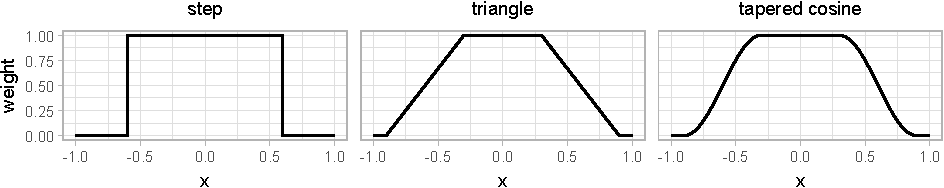
\includegraphics{manuscript_files/figure-latex/weighting-functions-1} 

}

\caption{Weighting functions investigated in this study to make power transformations more robust against outliers. In this example, the step function was parameterised with $\delta_1 = 0.60$. The triangle and tapered cosine functions were both parameterised with $\delta_1 = 0.30$ and $\delta_2 = 0.90$.}\label{fig:weighting-functions}
\end{figure}

Each weighting function has an argument \(\dot{x}\) that is related to
the (transformed) feature in one of several ways:

\begin{itemize}
\item
  The weighting function uses empirical probabilities of the
  distribution of the original feature \(\mathbf{X}\). After sorting
  \(\mathbf{X}\) in ascending order, probabilities are determined as
  \(p_i = \frac{i - 1/3}{n + 1/3}\), with \(i = 1, 2, \ldots n\), with
  \(n\) the number of instances of feature \(\mathbf{X}\). Then
  \(\dot{x}_i = p^{*}_i=2 \left( p_i - 0.5\right)\), so that argument is
  zero-centered.
\item
  The weighting function uses the z-score of the transformed feature
  \(\phi^{\lambda, x_0, s} (\mathbf{X})\). After Raymaekers and
  Rousseeuw (2024),
  \(z_i = \frac{\phi^{\lambda, x_0, s}(x_i) - \mu_M}{\sigma_M}\). Here,
  \(\mu_M\) and \(\sigma_M\) are robust Huber M-estimates of location
  and scale of the transformed feature
  \(\phi^{\lambda, x_0, s} (\mathbf{X})\) (Huber 1981). Then
  \(\dot{x}_i = z_i\).
\item
  After sorting \(\mathbf{X}\) in ascending order, the weighting
  function uses the residual error between the z-score of the
  transformed feature \(\phi^{\lambda, x_0, s} (\mathbf{X})\) and the
  theoretical z-score from a standard normal distribution:
  \(r_i =\left| \left( \phi^{\lambda, x_0, s}(x_i) - \mu_M)\right) / \sigma_M - F^{-1}_{\mathcal{N}}(p_i) \right|\),
  with \(\mu_M\), \(\sigma_M\) and \(p_i\) as defined above. Then
  \(\dot{x}_i = r_i\).
\end{itemize}

\subsection{Asymmetric generalised normal
distributions}\label{asymmetric-generalised-normal-distributions}

Modifications intended to make power transformations invariant to
location and scale of a feature and methods to improve their robustness
against outliers need to be assessed using data drawn from a range of
different distributions. Since the power transformations are intended
for use with unimodal distributions, the generalised normal distribution
(Subbotin 1923; Nadarajah 2005) is a suitable option for simulating
realistic feature distributions. This distribution has the following
probability density function \(f_{\beta}\) for a value
\(x \in \mathbb{R}\):

\begin{equation}
f_{\beta}(x) = \frac{\beta}{2\Gamma\left(1 / \beta \right)} e^{-\left| x \right|^\beta}
\end{equation}

Here, \(\Gamma\) is the gamma function, and \(\beta\) is a strictly
positive shape parameter. For \(\beta = 1\), the probability density
function describes a Laplace distribution. A normal distribution is
found for \(\beta=2\), and for large \(\beta\), the distribution
approaches a uniform distribution. We will refrain from introducing
scale and location parameters here directly.

Realistic feature distributions may be skewed. Gijbels et al.~describe a
recipe for introducing skewness into the otherwise symmetric generalised
normal distribution (Gijbels, Karim, and Verhasselt 2019), leading to
the following probability density function:

\begin{equation}
f_{\alpha}(x; \mu, \sigma, \beta) = \frac{2 \alpha \left(1 - \alpha\right)}{\sigma}
\begin{cases}
f_{\beta}\left( \left(1 - \alpha \right) \frac{\left| x - \mu \right|}{\sigma} \right) & \text{, } x \leq \mu \\
f_{\beta}\left( \alpha \frac{\left| x - \mu \right|}{\sigma} \right) & \text{, } x > \mu
\end{cases}
\end{equation}

Here, \(\alpha \in (0,1)\) is a skewness parameter. \(\alpha > 0.5\)
creates a distribution with a negative skew, i.e.~a left-skewed
distribution. A right-skewed distribution is created for
\(\alpha < 0.5\). \(\mu \in \mathcal{R}\) and \(\sigma \in (0, \infty)\)
are location and scale parameters, respectively. \(f_{\alpha}\) thus
describes the probability density function of an asymmetric generalised
normal distribution, which we will refer to here and parametrise as
\(\mathcal{AGN}\left(\mu, \sigma, \alpha, \beta \right)\).

We require a quantile function (or an approximation thereof) to draw
random values from an asymmetric generalised normal distribution using
inverse transform sampling. Gijbels et al.~derived the following
quantile function \(F_{\alpha}^{-1}(p)\):

\begin{equation}
F_{\alpha}^{-1}(p; \mu, \sigma, \beta) =
\begin{cases}
\mu + \frac{\sigma}{1 - \alpha} F_{\beta}^{-1} \left( \frac{p}{2 \alpha}\right) & \text{, } p \leq \alpha \\
\mu + \frac{\sigma}{\alpha} F_{\beta}^{-1} \left( \frac{1 + p - 2 \alpha}{2 \left(1 - \alpha \right)} \right) & \text{, } p > \alpha
\end{cases}
\end{equation}

The quantile function for the asymmetric generalised normal distribution
\(F_{\alpha}^{-1}\) thus incorporates the quantile function
\(F_{\beta}^{-1}\) of the symmetric generalised normal distribution.
\(F_{\beta}^{-1}\) was derived by Griffin to be (Griffin 2018):

\begin{equation}
F_{\beta}^{-1}(p) = \sgn\left(p - 0.5 \right) F_{\Gamma}^{-1}\left(2 \left|p - 0.5 \right|; 1 / \beta \right)
\end{equation}

Here, \(F_{\Gamma}^{-1}\) is the quantile function of the gamma
distribution with shape \(1 / \beta\), which can be numerically
approximated.

\subsection{Empirical central normality
test}\label{empirical-central-normality-test}

Power transformations aim to transform features to a normal
distribution. However, this may not always be successful or possible.
Deviations from normality can be detected by normality tests, such as
the Shapiro-Wilk test (Shapiro and Wilk 1965). In practice, normality
tests may be too stringent with large sample sizes, outliers, or both.
Here we develop an empirical test for central normality. The null
hypothesis \(H_0\) is that the distribution is centrally normal. The
alternative hypothesis \(H_1\) is that the distribution is not centrally
normal.

Let central normality be defined as the normality of central portion
\(\kappa\) of the data,
i.e.~\(\mathbf{X}_{\text{central}} = \left\{x_i \in \mathbf{X} \, | \,  \frac{1-\kappa}{2} \leq  p_i \leq \frac{1 + \kappa}{2}\right\}\),
with \(p_i\) probabilities of the empirical distribution, as previously.
We then compute the residual errors between the z-scores of the
transformed feature \(\phi^{\lambda, x_0, s} (\mathbf{X})\) and the
expected z-scores from a standard normal distribution:
\(r_i =\left| \left( \phi^{\lambda, x_0, s}(x_i) - \mu_M)\right) / \sigma_M - F^{-1}_{\mathcal{N}}(p_i) \right|\),
with \(\mu_M\) and \(\sigma_M\) robust Huber M-estimates of location and
scale of the transformed feature \(\phi^{\lambda, x_0, s} (\mathbf{X})\)
(Huber 1981). The set of residual errors for the central portion of the
data is then
\(\mathbf{R}_{\text{central}} = \left\{ r_i \in \left\{ r_1, r_2, \ldots, r_n\right\} \, | \,  \frac{1-\kappa}{2} \leq  p_i \leq \frac{1 + \kappa}{2}\right\}\).

The test statistic \(\tau_{\text{ecn}}\) is then defined as:

\begin{equation}
\tau_{\text{ecn}} = \frac{\sum_{i=1}^{N} r_i \left[r_i \in \mathbf{R}_{\text{central}}\right]}{\sum_{i=1}^N \left[r_i \in \mathbf{R}_{\text{central}}\right]} 
\end{equation}

Here \([\quad]\) denotes an Iverson bracket. The test statistic is equal
to the mean of the residual errors of the central portion of the data.

To use the test statistic, the central portion of the data needs to be
defined and the Type 1 error rates determined. We will do so in the
\hyperref[simulation]{Simulation} section.

\section{Simulation}\label{simulation}

We used simulated data to assess invariance to location and scale of the
proposed power transformations, weighting for robust transformations,
and to develop the empirical central normality test. The \(\lambda\)
parameter for conventional power transformations (Eqn.
\ref{eqn:box-cox-original} and \ref{eqn:yeo-johnson-original}), as well
as \(\lambda\), \(x_0\) and \(s\) parameters for location- and
scale-invariant power transformations (Eqn. \ref{eqn:box-cox-invariant}
and \ref{eqn:yeo-johnson-invariant}) were estimated using the BOBYQA
algorithm for derivative-free bound constraint optimisation (Powell
2009) through maximum likelihood estimation. The required algorithms
were implemented in the \texttt{power.transform} R software package
(Zwanenburg and Löck 2024b) (version 1.0.0). Of note, the
\texttt{power.transform} package shifts feature values into the positive
domain if negative or zero values are present for Box-Cox power
transformations.

\subsection{Invariance to location and
scale}\label{invariance-to-location-and-scale}

To assess whether the proposed power transformations lead to values of
\(\lambda\) that are invariant to location and scale of the
distribution, we simulated three different distributions. We first
randomly drew \(10000\) values from a normal distribution:
\(\mathbf{X}_{\text{normal}} = \left\{x_1, x_2, \ldots, x_{10000} \right\} \sim \mathcal{N}\left(0, 1\right)\),
or equivalently
\(\mathbf{X}_{\text{normal}} = \left\{x_1, x_2, \ldots, x_{10000} \right\} \sim \mathcal{AGN}\left(0, 1/\sqrt{2}, 0.5, 2\right)\).
The second distribution was a right-skewed generalised normal
distribution
\(\mathbf{X}_{\text{right}} = \left\{x_1, x_2, \ldots, x_{10000} \right\} \sim \mathcal{AGN}\left(0, 1/\sqrt{2}, 0.2, 2\right)\).
The third distribution was a left-skewed generalised normal distribution
\(\mathbf{X}_{\text{left}} = \left\{x_1, x_2, \ldots, x_{10000} \right\} \sim \mathcal{AGN}\left(0, 1/\sqrt{2}, 0.8, 2\right)\).
We then computed transformation parameter \(\lambda\) using the original
definitions (Eqn. \ref{eqn:box-cox-original} and
\ref{eqn:yeo-johnson-original}) and the location- and scale-invariant
definitions (Eqn. \ref{eqn:box-cox-invariant} and
\ref{eqn:yeo-johnson-invariant}) for each distribution. To assess
location invariance, a positive value \(d_{\text{shift}}\) was added to
each distribution with \(d_{\text{shift}} \in [1, 10^6]\). Similarly, to
assess scale invariance, each distribution was multiplied by a positive
value \(d_{\text{scale}}\), where \(d_{\text{scale}} \in [1, 10^6]\).

\begin{figure}

{\centering 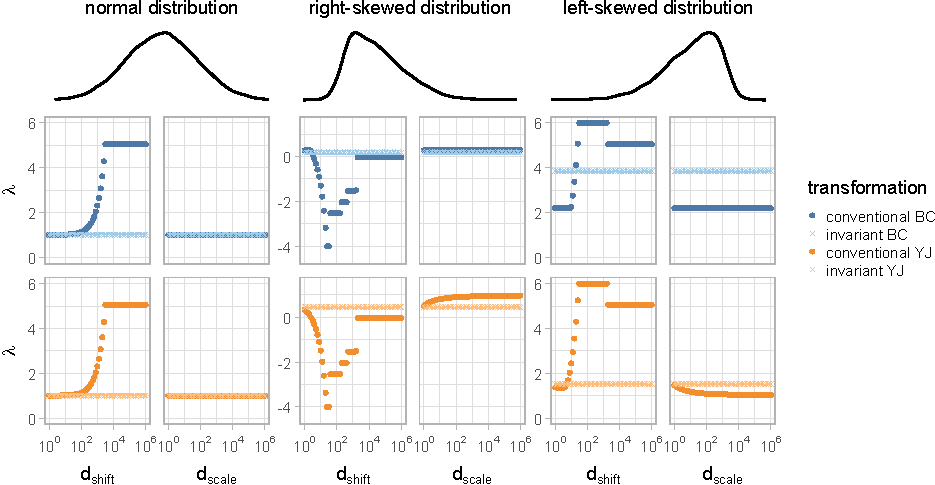
\includegraphics{manuscript_files/figure-latex/shifted-distributions-1} 

}

\caption{Invariant power transformation produces transformation parameters that are invariant to location and scale. Samples were drawn from normal, right-skewed and left-skewed distributions, respectively, which then underwent a shift $d_{\text{shift}}$ or multiplication by $d_{\text{scale}}$. Estimates of the transformation parameter $\lambda$ for the conventional power transformations show strong dependency on the overall location and scale of the distribution, whereas estimates obtained for the location- and scale-invariant power transformations are constant.}\label{fig:shifted-distributions}
\end{figure}

The result is shown in Figure \ref{fig:shifted-distributions}. For each
distribution, transformation parameter \(\lambda\) varied with
\(d_{\text{shift}}\) and \(d_{\text{scale}}\) when estimated for
conventional transformations. In contrast, estimation of \(\lambda\) for
invariant power transformations was invariant to both
\(d_{\text{shift}}\) and \(d_{\text{scale}}\).

\subsection{Robust transformations}\label{robust-transformations}

Outliers may be present in data and affect estimation of transformation
parameters. The log-likelihood function can be weighted to assign less
weight to outlier instances, see equations
\ref{eqn:box-cox-weighted-invariant-log-likelihood} and
\ref{eqn:yeo-johnson-weighted-invariant-log-likelihood}. We proposed
three weighting function: step, triangle and tapered cosine, that have
one, two and two parameters, respectively. Each weighting function then
takes one of three values as input: probabilities of the empirical
distribution of the original feature, the z-score of the transformed
feature values, or the residual error between the z-score of the
transformed feature values and their expected z-score based on the
normal distribution.

To determine the weighting function parameters for each of the nine
combinations, \(m_d=100\) asymmetric generalised normal distributions
were drawn. Each distribution was parametrised with a randomly chosen
skewness parameter \(\alpha \sim U\left(0.01, 0.99\right)\) and shape
parameter \(\beta \sim U\left(1.00, 5.00 \right)\). Location and scale
parameters were set as \(\mu = 0\) and \(\sigma = 1\), respectively.
\(n = \lceil 10^\gamma \rceil\) instances were then randomly drawn, with
\(\gamma \sim U\left(2, 4\right)\), i.e., between \(100\) and \(10000\)
values are drawn to create \(\mathbf{X}_i\).

Outlier values were then drawn to randomly replace a fraction of the
values of \(\mathbf{X}_i\). This was repeated \(m_{\text{out}} = 10\)
times, with outlier fractions regularly spaced in \([0.00, 0.10]\). Thus
up to 10 percent of the values could be replaced by outliers. Outlier
values were set according to John W. Tukey (1977), as follows. Let
\(x^{*} \sim U\left(-2, 2\right)\). Then the corresponding outlier value
was:

\begin{equation}
x_{out} =
\begin{cases}
Q_1 - \left(1.5 - x^{*} \right) \text{IQR} & \text{if } x^{*} < 0 \\
Q_3 + \left(1.5 + x^{*} \right) \text{IQR} & \text{if } x^{*} \geq 0
\end{cases}
\end{equation}

\(Q_1\), \(Q_3\) and \(\text{IQR}\) are the first quartile, third
quartile and interquartile range of \(\mathbf{X}_i\), respectively.
Outlier values randomly replaced values in \(\mathbf{X}_i\) to create
\(\mathbf{X}_{i,j}\), with
\(j \in \left\{ 1, \ldots, m_{\text{out}} \right\}\)

To find the optimal values for the weighting function parameters
\(\delta_1\) and \(\delta_2\) (if applicable), we minimised the absolute
difference between the \(\lambda_{r}\) parameter obtained for robust
transformation in the presence of outliers, and the \(\lambda_0\)
parameter obtained using the non-robust transformations in absence of
outliers:

\begin{equation}
\label{eqn:minimisation-weighting}
\left\{ \hat{\delta}_1, \hat{\delta}_2 \right\} = \argmin_{\delta_1, \delta_2} \sum_{i=1}^{m_d} \sum_{j=1}^{m_{\text{out}}} \left| \lambda_r \left(\mathbf{X}_{i, j}; \delta_1, \delta_2 \right) - \lambda_0 \left(\mathbf{X}_i \right) \right|
\end{equation}

Minimisation was conducted using the BOBYQA algorithm for
derivative-free bound constraint optimisation (Powell 2009). The
resulting weighting function parameters for weighted MLE are shown in
Tables \ref{tab:optimal-weighting-parameters-box-cox} and
\ref{tab:optimal-weighting-parameters-yeo-johnson} for robust location-
and scale-invariant Box-Cox and Yeo-Johnson transformations,
respectively.

\begin{table}
\begin{center}
\caption{Optimal weighting parameters and corresponding loss for location- and scale-invariant Box-Cox power transformations. $p^{*}$ indicates use of the empirical distribution of feature values, $z$ the z-score of the transformed feature values, and $r$ the residual error between the z-score of transformed feature values and the expected z-score according to the normal distribution. The \textit{initial} column shows the starting parameter value for the optimisation process, with the corresponding boundary values in the \textit{limits} column. The {optimal} column shows the optimal parameter values. The \textit{loss} column shows the loss achieved by each method, under optimised parameters. Lower loss indicates better robustness against outliers.}
\label{tab:optimal-weighting-parameters-box-cox}
\begin{tabular}{l r r r r r r r}

\toprule
method & \multicolumn{3}{c}{$\delta_1$} & \multicolumn{3}{c}{$\delta_2$} & loss \\
& initial & limits & optimal & initial & limits & optimal & \\

\midrule
non-robust               & ---  & ---       & ---  & ---  & ---       & ---  & 771 \\
$p^{*}$ (step)           & 0.80 & $(0, 1]$  & 0.86 & ---  & ---       & ---  & 561 \\
$p^{*}$ (triangle)       & 0.80 & $(0, 1]$  & 0.83 & 0.95 & $(0, 1]$  & 0.92 & 564 \\
$p^{*}$ (tapered cosine) & 0.80 & $(0, 1]$  & 0.76 & 0.95 & $(0, 1]$  & 0.95 & 560 \\
$z$ (step)               & 1.28 & $(0, 10]$ & 1.12 & ---  & ---       & ---  & 1153 \\
$z$ (triangle)           & 1.28 & $(0, 10]$ & 0.38 & 1.96 & $(0, 10]$ & 4.48 & 1178 \\
$z$ (tapered cosine)     & 1.28 & $(0, 10]$ & 1.21 & 1.96 & $(0, 10]$ & 4.92 & 1135 \\
$r$ (step)               & 0.50 & $(0, 10]$ & 2.18 & ---  & ---       & ---  & 1839 \\
$r$ (triangle)           & 0.50 & $(0, 10]$ & 1.29 & 1.00 & $(0, 10]$ & 1.47 & 1764 \\
$r$ (tapered cosine)     & 0.50 & $(0, 10]$ & 1.38 & 1.00 & $(0, 10]$ & 1.41 & 1583 \\
\bottomrule
\end{tabular}
\end{center}
\end{table}

\begin{table}
\begin{center}
\caption{Optimal weighting parameters and corresponding loss for location- and scale-invariant Yeo-Johnson power transformations. $p^{*}$ indicates use of the empirical distribution of feature values, $z$ the z-score of the transformed feature values, and $r$ the residual error between the z-score of transformed feature values and the expected z-score according to the normal distribution. The \textit{initial} column shows the starting parameter value for the optimisation process, with the corresponding boundary values in the \textit{limits} column. The {optimal} column shows the optimal parameter values. The \textit{loss} column shows the loss achieved by each method, under optimised parameters. Lower loss indicates better robustness against outliers.}
\label{tab:optimal-weighting-parameters-yeo-johnson}
\begin{tabular}{l r r r r r r r}

\toprule
method & \multicolumn{3}{c}{$\delta_1$} & \multicolumn{3}{c}{$\delta_2$} & loss \\
& initial & limits & optimal & initial & limits & optimal & \\

\midrule
non-robust               & ---  & ---       & ---  & ---  & ---       & ---  & 364 \\
$p^{*}$ (step)           & 0.80 & $(0, 1]$  & 0.95 & ---  & ---       & ---  & 224 \\
$p^{*}$ (triangle)       & 0.80 & $(0, 1]$  & 0.88 & 0.95 & $(0, 1]$  & 0.97 & 212 \\
$p^{*}$ (tapered cosine) & 0.80 & $(0, 1]$  & 0.94 & 0.95 & $(0, 1]$  & 0.95 & 218 \\
$z$ (step)               & 1.28 & $(0, 10]$ & 1.09 & ---  & ---       & ---  & 392 \\
$z$ (triangle)           & 1.28 & $(0, 10]$ & 0.24 & 1.96 & $(0, 10]$ & 4.62 & 396 \\
$z$ (tapered cosine)     & 1.28 & $(0, 10]$ & 0.15 & 1.96 & $(0, 10]$ & 6.05 & 413 \\
$r$ (step)               & 0.50 & $(0, 10]$ & 1.63 & ---  & ---       & ---  & 746 \\
$r$ (triangle)           & 0.50 & $(0, 10]$ & 1.50 & 1.00 & $(0, 10]$ & 1.79 & 731 \\
$r$ (tapered cosine)     & 0.50 & $(0, 10]$ & 1.51 & 1.00 & $(0, 10]$ & 1.57 & 612 \\
\bottomrule
\end{tabular}
\end{center}
\end{table}

Figure \ref{fig:optimised-weighting-function-parameters} shows the
distribution of errors \(\left| \lambda_r - \lambda_0 \right|\) for
non-robust and robust transformations using the optimal weighting
function parameters. In the presence of outliers, the Yeo-Johnson
transformation yielded smaller errors than the Box-Cox transformation.
For both transformations, weighting based on empirical probabilities
yielded the most consistent \(\lambda\) parameter estimates in the
presence of outliers. Other methods did not outperform the non-robust
transformation method.

\begin{figure}

{\centering 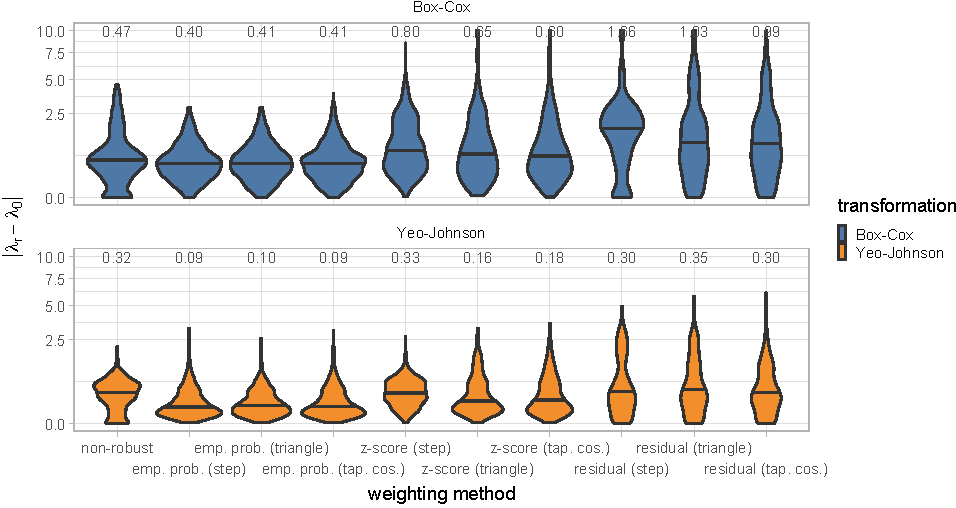
\includegraphics{manuscript_files/figure-latex/optimised-weighting-function-parameters-1} 

}

\caption{Robustness of power transformations after optimising weighting function parameters. The distribution of errors, i.e. the difference between robustly fitted $\lambda^r$ and expected $\lambda_{0}$ found in the absence of outliers, is shown for 1000 randomly parametrised asymmetric generalised normal distributions with up to 10\% outliers on either side of the distribution. The top and bottom panel show errors for the location- and scale-invariant Box-Cox and Yeo-Johnson transformations, respectively. In each panel, the error distribution for the non-robust transformation is shown to the left for comparison with different weighting methods. Note that a square root transformation was applied along the $y$-axis for display purposes. Median errors are shown above each distribution.}\label{fig:optimised-weighting-function-parameters}
\end{figure}

\subsection{Empirical central normality
test}\label{empirical-central-normality-test-1}

To develop an empirical test for central normality we need to consider
two parameters: the central portion \(\kappa\) as a fixed parameter, and
test statistic \(\tau_{\text{ecn}}\). We will first define the central
portion \(\kappa\).

First we draw \(m_d=10000\) random asymmetric generalised normal
distributions. As before, each distribution is parametrised with a
randomly chosen skewness parameter
\(\alpha \sim U\left(0.01, 0.99\right)\) and shape parameter
\(\beta \sim U\left(1.00, 5.00 \right)\). Location and scale parameters
are set as \(\mu = 0\) and \(\sigma = 1\), respectively.
\(n = \lceil 10^\gamma \rceil\) values are then randomly drawn, with
\(\gamma \sim U\left(1.47, 3.00\right)\), which leads to between \(30\)
and \(1000\) values being drawn to create \(\mathbf{X}_i\). As before,
for each distribution, up to \(10 \%\) of instances are replaced by
outlier values, and this is repeated \(10\) times. We then compute
residuals after optimising robust location- and scale-invariant
transformations with the empirical tapered cosine weighting method.

Figure \ref{fig:empirical-central-normality-residual-error} shows the
residual errors of the transformed distribution as function of the
empirical probability. As expected, the largest deviations from
normality appear on the extremities of this range. For Box-Cox
transformations, the effect of outliers on the lower end of the
distribution leads to noticeable asymmetry. Between very low and very
high empirical probabilities, residual errors are constrained and
relatively flat. This is the candidate range for the central portion of
the data.

\begin{figure}

{\centering 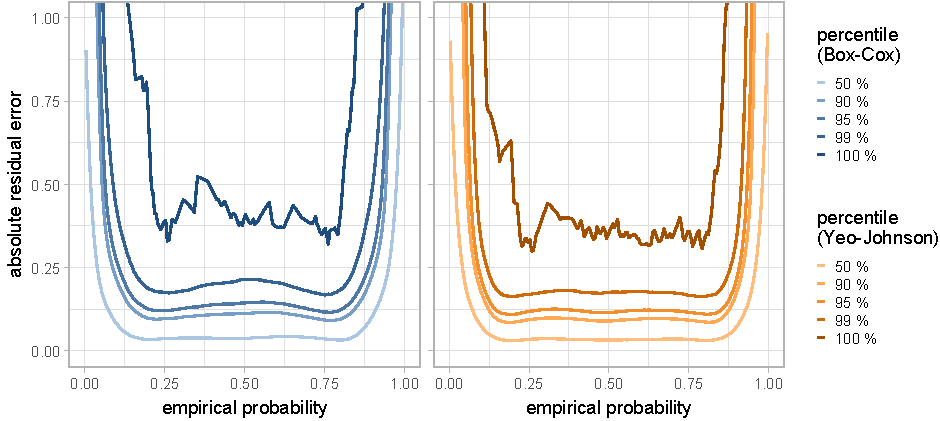
\includegraphics{manuscript_files/figure-latex/empirical-central-normality-residual-error-1} 

}

\caption{Residual error as a function of empirical probability. Percentiles of the error are shown for robust, location- and scale-invariant transformations of 10000 randomly drawn asymmetric generalised normal distributions, for each of which outliers were randomly drawn 10 times (up to 10\% of samples). Larger errors occur at the edges of each distribution.}\label{fig:empirical-central-normality-residual-error}
\end{figure}

We then consider the empirical probability of type I errors: the
probability of incorrectly classifying a centrally normal distribution
as being non-normal based on the test statistic \(\tau_{\text{ecn}}\).
Under the assumption that the asymmetric generalised normal
distributions are centrally normal after robust transformation, this
produces the relationship shown in Figure
\ref{fig:empirical-central-normality-type-1-error-rate}. Since for
\(\kappa \leq 0.80\) error curves for both transformation methods are
similar, we fix the value of the central portion \(\kappa\) to 0.80. In
the remaining we will use the empirical central normality test statistic
values defined using robust location- and scale-invariant Yeo-Johnson
transformations, as it is more conservative (see Appendix E). This leads
to test statistic values listed in Table
\ref{tab:empirical-central-normality}

\begin{figure}

{\centering 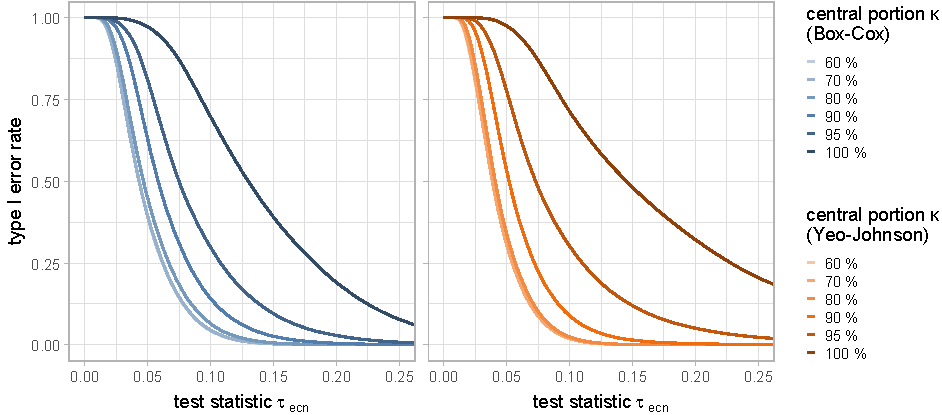
\includegraphics{manuscript_files/figure-latex/empirical-central-normality-type-1-error-rate-1} 

}

\caption{Type 1 error rate of transformed asymmetric generalised normal distributions as function of the test statistic $\tau_{\text{ecn}}$ for the central portion $\kappa$ of the distribution.}\label{fig:empirical-central-normality-type-1-error-rate}
\end{figure}

\begin{table}
\begin{center}
\caption{Test statistic $\tau_{\text{ecn}}$ for empirical central normality at $\kappa = 0.80$ as a function of Type I error rate.}
\label{tab:empirical-central-normality}
\begin{tabular}{l | c c c c c c c}

\toprule
type I error rate & 0.50 & 0.20 & 0.10 & 0.05 & 0.02 & 0.01 & 0.001 \\

\midrule
$\tau_{\text{ecn}}$ & 0.041 & 0.062 & 0.075 & 0.088 & 0.103 & 0.115 & 0.154 \\
\bottomrule
\end{tabular}
\end{center}
\end{table}

In Figure \ref{fig:empirical-central-normality-examples} we apply the
empirical central normality test to assess central normality of features
that are composed of a mixture of samples drawn from two normal
distributions. With increased separation of the underlying normal
distributions, the probability of the feature being centrally normal
decreases, as expected.

\begin{figure}

{\centering 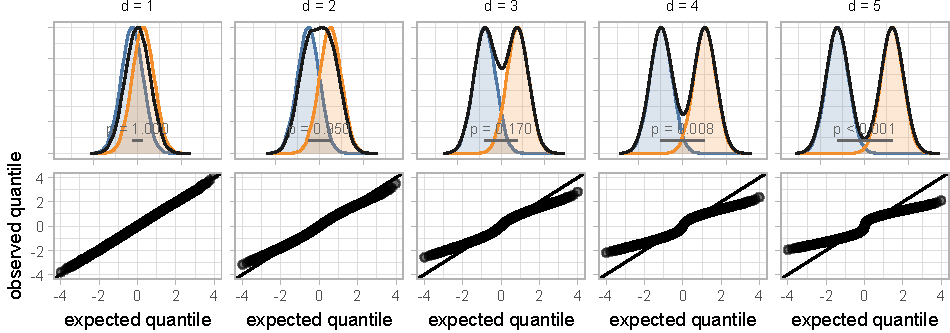
\includegraphics{manuscript_files/figure-latex/empirical-central-normality-examples-1} 

}

\caption{Bi-modal distributions and empirical central normality test results. The feature (black) is a mixture of two identical sample sets (blue and orange) drawn from normal distributions that are offset by a distance $d$. We use the empirical centrally normality test to compute the probability for the hypothesis that the distribution is centrally normal. As may be observed, with increasing offset $d$ the probability that the feature is centrally normal decreases. Quantile-quantile plots are drawn below each distribution.}\label{fig:empirical-central-normality-examples}
\end{figure}

\section{Experimental Results}\label{experimental-results}

\subsection{Invariance}\label{invariance}

Location- and scale-invariant power transformations are intended to
yield improved transformations to normality in the presence of large
shifts in location, distributions that due to location and scale are not
centered near zero, or both. Earlier, we assessed these transformations
using simulated data. In the following, they are evaluated using
examples from real datasets. We focus on the Yeo-Johnson transformation
because of its ability to handle features with negative values. Results
for Box-Cox transformations are shown in Appendix D.

\begin{figure}

{\centering 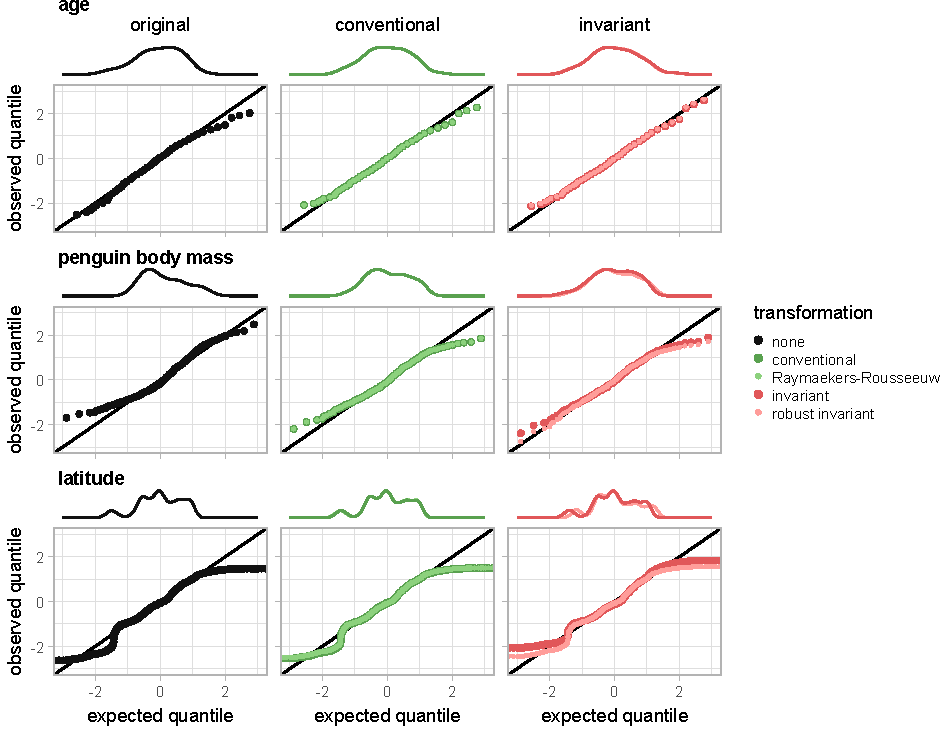
\includegraphics{manuscript_files/figure-latex/experimental-results-invariance-1} 

}

\caption{Quantile-quantile plots for several datasets: age of patients with lung cancer (top row); penguin body mass (middle row); and latitude coordinates of houses sold in Ames, Iowa (bottom row). Multiple quantile-quantile plots are shown: for the original feature (left column); the feature transformed using the conventional Yeo-Johnson transformation and Raymaekers and Rousseeuw's robust adaptation (middle column); and the feature transformed using the non-robust and robust location- and-scale invariant Yeo-Johnson transformations (right column).}\label{fig:experimental-results-invariance}
\end{figure}

\subsubsection{Age of patients with lung
cancer}\label{age-of-patients-with-lung-cancer}

A common feature in health-related datasets is age. Here we use data on
228 patients with lung cancer that was collected and published by
Loprinzi et al. (Loprinzi et al. 1994). The age in the cohort was
\(62.4 \pm 9.1\) (mean ± standard deviation) years. Applying
conventional and invariant Yeo-Johnson transformations to patient age
yielded the following results, see Figure
\ref{fig:experimental-results-invariance}: no transformation (sum of
residuals with normal distribution \(\sum r_i = 16.5\)); conventional
transformation (\(\lambda = 2.0\), \(\sum r_i = 11.5\),
\(\mu_{YJ} = 1.8 \cdot 10^3\), \(\sigma_{YJ} = 0.5 \cdot 10^3\));
Raymaekers and Rousseeuw's robust adaptation (\(\lambda = 2.0\),
\(\sum r_i = 11.5\), \(\mu_{YJ} = 1.8 \cdot 10^3\),
\(\sigma_{YJ} = 0.5 \cdot 10^3\)); location- and scale-invariant
transformation (\(\lambda = 0.9\), \(\sum r_i = 8.8\),
\(\mu_{YJ} = 1.2\), \(\sigma_{YJ} = 1.1\)); and robust location- and
scale-invariant transformation (\(\lambda = 0.8\), \(\sum r_i = 10.6\),
\(\mu_{YJ} = 1.2\), \(\sigma_{YJ} = 1.0\)).

Location- and scale-invariant transformation led to a lower overall
residual sum, indicating a better transformation. Robust location- and
scale-invariant transformation had a higher residual sum compared to the
non-robust variant, which may be due to the lack of outliers in the
data. Conventional transformations inflated the mean \(\mu_{YJ}\) and
standard deviation \(\sigma_{YJ}\) of the age feature after
transformation. The empirical central normality test did not detect any
statistically significant deviations from central normality for any
transformation (all \(p \geq 0.78\)).

\subsubsection{Penguin body mass}\label{penguin-body-mass}

Gorman, Williams and Fraser recorded body mass (in grams) of 342
penguins of three different species (Gorman, Williams, and Fraser 2014).
The body mass was \((4.2 \pm 0.8) \cdot 10^3\) (mean ± standard
deviation) grams, and not centrally normal (\(p = 0.03\)). Applying
conventional and invariant Yeo-Johnson transformations to body mass
yielded the following results, see Figure
\ref{fig:experimental-results-invariance}: no transformation (residual
sum \(\sum r_i = 48.0\)); conventional transformation
(\(\lambda = -0.5\), \(\sum r_i = 32.2\), \(\mu_{YJ} = 2.1\),
\(\sigma_{YJ} = 4 \cdot 10^{-3}\)); Raymaekers and Rousseeuw's robust
adaptation (\(\lambda = -0.5\), \(\sum r_i = 32.2\), \(\mu_{YJ} = 2.1\),
\(\sigma_{YJ} = 4 \cdot 10^{-3}\)); location- and scale-invariant
transformation (\(\lambda = 0.5\), \(\sum r_i = 26.8\),
\(\mu_{YJ} = 0.9\), \(\sigma_{YJ} = 0.9\)); and robust location- and
scale-invariant transformation (\(\lambda = 0.4\), \(\sum r_i = 23.1\),
\(\mu_{YJ} = 0.8\), \(\sigma_{YJ} = 0.8\)).

Location- and scale-invariant transformation produced a lower overall
residual sum, indicating a better transformation. Moreover, conventional
transformations led to low standard deviation \(\sigma_{YJ}\) of the
body mass feature after transformation. The empirical central normality
test did not detect any statistically significant deviations from
central normality for any transformation (all \(p \geq 0.38\)).

\subsubsection{Latitude in the Ames housing
dataset}\label{latitude-in-the-ames-housing-dataset}

Geospatial datasets usually contain coordinates. The Ames housing
dataset contains data on 2930 properties that were sold between 2006 and
2010 (De Cock 2011), including their geospatial coordinates. The
latitude was \(42.03 \pm 0.02)\) (mean ± standard deviation). Applying
conventional and invariant Yeo-Johnson transformations to latitude
yielded the following results, see Figure
\ref{fig:experimental-results-invariance}: no transformation (residual
sum \(\sum r_i = 328\)); conventional transformation
(\(\lambda = 62.1\), \(\sum r_i = 319\),
\(\mu_{YJ} = 4.8 \cdot 10^{99}\), \(\sigma_{YJ} = 0.1 \cdot 10^{99}\));
Raymaekers and Rousseeuw's robust adaptation (\(\lambda = 95.4\),
\(\sum r_i = 319\), \(\mu_{YJ} = 6.4 \cdot 10^{153}\),
\(\sigma_{YJ} = 0.3 \cdot 10^{153}\)); location- and scale-invariant
transformation (\(\lambda = 1.5\), \(\sum r_i = 326\),
\(\mu_{YJ} = -1.2\), \(\sigma_{YJ} = 0.8\)); and robust location- and
scale-invariant transformation (\(\lambda = 1.4\), \(\sum r_i = 311\),
\(\mu_{YJ} = -1.3\), \(\sigma_{YJ} = 0.9\)).

Every transformation reduced the residual sum. The non-robust location-
and scale-invariant transformation did not improve over conventional
alternatives and yielded a data distribution lacking central normality
(empirical central normality test: \(p=0.05\)). However, conventional
transformations had high values for the \(\lambda\) parameter, which
could lead to numerical issues.

\subsection{Robustness against
outliers}\label{robustness-against-outliers}

We previously simulated data to assess invariant power transformations
and their robustness against outliers. Here, we assess invariant power
transformations in real data with outliers.

\begin{figure}

{\centering 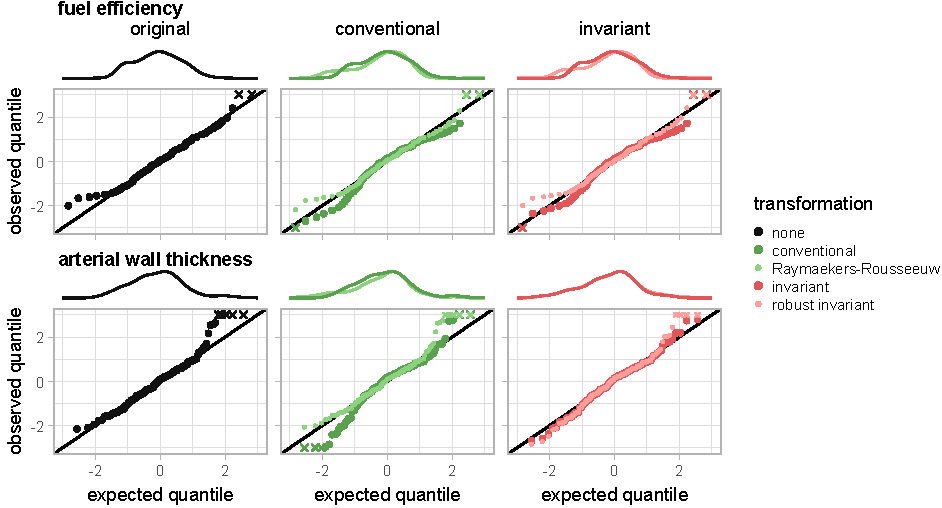
\includegraphics{manuscript_files/figure-latex/experimental-results-outlier-robustness-1} 

}

\caption{Quantile-quantile plots for two datasets with outliers: vehicle fuel consumption (top row), where outliers are related to highly fuel-efficient vehicles; and maximum arterial wall thickness in patients with ischemic stroke (bottom row). Multiple quantile-quantile plots are shown: for the original feature (left column); the feature transformed using the conventional Yeo-Johnson transformation and Raymaekers and Rousseeuw's robust adaptation (middle column); and the feature transformed using the non-robust and robust location- and-scale invariant Yeo-Johnson transformations (right column). Samples with observed quantiles below $-3.0$ or above $3.0$ are indicated by crosses.}\label{fig:experimental-results-outlier-robustness}
\end{figure}

\subsubsection{Fuel efficiency in the Top Gear
dataset}\label{fuel-efficiency-in-the-top-gear-dataset}

The Top Gear dataset contains data on 297 vehicles that appeared on the
BBC television show \emph{Top Gear} (Alfons 2021). Within this dataset,
the fuel consumption feature contains outliers due to highly
fuel-efficient vehicles. Applying conventional and invariant Yeo-Johnson
transformations to the fuel consumption feature yielded the following
results, see Figure \ref{fig:experimental-results-outlier-robustness}:
no transformation (residual sum \(\sum r_i = 54\), \(p=0.76\));
conventional transformation (\(\lambda = -0.1\), \(\sum r_i = 55\),
\(\mu_{YJ} = 3.0\), \(\sigma_{YJ} = 0.3\), \(p=0.01\)); Raymaekers and
Rousseeuw's robust adaptation (\(\lambda = 0.8\), \(\sum r_i = 48\),
\(\mu_{YJ} = 29\), \(\sigma_{YJ} = 15\), \(p=0.55\)); location- and
scale-invariant transformation (\(\lambda = -1.3\), \(\sum r_i = 44\),
\(\mu_{YJ} = 0.5\), \(\sigma_{YJ} = 0.1\), \(p=0.03\)); and robust
location- and scale-invariant transformation (\(\lambda = -0.9\),
\(\sum r_i = 50\), \(\mu_{YJ} = 2.0\), \(\sigma_{YJ} = 2.3\),
\(p=0.58\)).

Outliers cause non-robust transformations to fail to transform the data
to a centrally normal distribution (empirical central normality test
\(p = 0.01\) and \(p=0.03\) for conventional and invariant
transformations, respectively). Robust transformations produce
distributions that are centrally normal (empirical central normality
test \(p > 0.05\)).

\subsubsection{Maximum arterial wall thickness in an ischemic stroke
dataset}\label{maximum-arterial-wall-thickness-in-an-ischemic-stroke-dataset}

The ischemic stroke dataset contains historic data from 126 patients
with risk at ischemic stroke (Kuhn and Johnson 2019). These patients
underwent Computed Tomography Angiography to characterize the carotid
artery blockages. Angiography imaging was then assessed, and various
characteristics related to the blood vessels and the disease are
measured. The maximum arterial wall thickness feature contains several
instances with outlier values. Applying conventional and invariant
Yeo-Johnson transformations to this feature yielded the following
results, see Figure \ref{fig:experimental-results-outlier-robustness}:
no transformation (residual sum \(\sum r_i = 110\), \(p=0.56\));
conventional transformation (\(\lambda = -0.7\), \(\sum r_i = 30\),
\(\mu_{YJ} = 1.0\), \(\sigma_{YJ} = 0.1\), \(p=0.01\)); Raymaekers and
Rousseeuw's robust adaptation (\(\lambda = 1.1\), \(\sum r_i = 136\),
\(\mu_{YJ} = 7.2\), \(\sigma_{YJ} = 14\), \(p=0.61\)); location- and
scale-invariant transformation (\(\lambda = 0.2\), \(\sum r_i = 12\),
\(\mu_{YJ} = -11.8\), \(\sigma_{YJ} = 6.9\), \(p=0.13\)); and robust
location- and scale-invariant transformation (\(\lambda = -0.6\),
\(\sum r_i = 27\), \(\mu_{YJ} = 0.7\), \(\sigma_{YJ} = 0.1\),
\(p=0.10\)).

Non-robust transformations failed to produce a centrally normal
distribution (empirical central normality test \(p=0.01\) and \(p=0.02\)
for conventional and invariant transformations, respectively). Robust
transformations produce distributions that are centrally normal
(empirical central normality test \(p > 0.05\)).

\subsection{Integration into end-to-end machine
learning}\label{integration-into-end-to-end-machine-learning}

We used 285 datasets from the Penn Machine Learning Benchmarks
collection (Romano et al. 2022). In this collection, 122 datasets
correspond to regression tasks and 163 datasets to classification tasks.
Using the familiar auto-machine learning library (Zwanenburg and Löck
2024a) (version 1.5.0), each dataset was used to train a model for each
of 16 process configurations. Each process configuration specifies the
learner (generalised linear model or random forest), transformation
method (none, conventional Yeo-Johnson, robust invariant Yeo-Johnson,
robust invariant Yeo-Johnson with empirical central normality test
(rejecting transformations with \(p \leq 0.01\)), and normalisation
method (none, \(z\)-standardisation), yielding 16 distinct
configurations. Before each experiment, each dataset was randomly split
into a training (70\%) and holdout test (30\%) set five times. Thus, a
total of 22800 models were created. Each model was then evaluated using
the holdout test set using one of two metrics, i.e.~the root relative
squared error (RRSE) for regression tasks and the area under the
receiver operating characteristic curve (AUC) for classification tasks.

For the purpose of assessing the effect of the difficulty of the task,
we computed the median performance score over all models for each
dataset and assigned one the following categories:

\begin{itemize}
\tightlist
\item
  very easy: \(\text{AUC} \geq 0.90\) or \(\text{RRSE} \leq 0.10\) (87
  datasets)
\item
  easy: \(0.90 > \text{AUC} \geq 0.80\) or
  \(0.30 \geq \text{RRSE} > 0.10\) (46 datasets)
\item
  intermediate: \(0.80 > \text{AUC} \geq 0.70\) or
  \(0.60 \geq \text{RRSE} > 0.30\) (72 datasets)
\item
  difficult: \(0.70 > \text{AUC} \geq 0.60\) or
  \(0.80 \geq \text{RRSE} > 0.60\) (60 datasets)
\item
  very difficult: \(0.60 > \text{AUC} \geq 0.50\) or
  \(1.00 \geq \text{RRSE} > 0.80\) (12 datasets)
\item
  unsolvable: \(\text{AUC} < 0.50\) or \(\text{RRSE} > 1.00\) (8
  datasets)
\end{itemize}

To remove the effect of the dataset, and allow for comparing metrics, we
ranked all performance scores for each dataset so that a higher rank
corresponds to better performance. Experiments yielding the same score
received the same, average, rank. Subsequently ranks were normalised to
the \([0.0, 1.0]\) range.

Significant differences exist between process configurations (Friedman
test: \(p < 10^{-8})\).

Here we focus on the subset of 232 datasets that contain numeric
features. Considering single process parameters, the choice of learner
(Wilcoxon signed rank test: \(p < 10^{-8})\)) and normalisation method
(Wilcoxon signed rank test: \(p = 0.007\)) had a significant impact (at
significance level \(p = 0.050\)), but transformation method (Friedman
test: \(p = 0.054\)) did not.

To estimate the marginal effects of process parameters, including
transformation method, we first fit a regression random forest (ranger
package (Wright and Ziegler 2017) version 0.16.0): 2000 trees, minimum
node size 2, other hyperparameters default) with process parameters and
task difficulty as predictors and normalised rank as response variable.
The estimated marginal effects are shown in Figure
\ref{fig:marginal-effect-plot}. On the scale of normalised ranks
(\([0.0, 1.0]\)), the overall estimated marginal effect of using a
random forest instead of generalised linear model was \(0.272\). The
overall marginal effect of using z-standardisation to normalise features
was \(0.008\). Transformation methods had the following marginal
effects: \(0.003\) for using conventional Yeo-Johnson transformation
instead of no transformation; \(-0.007\) for using robust invariant
Yeo-Johnson transformation instead of no transformation; \(-0.009\) for
using robust invariant Yeo-Johnson transformation with empirical central
normality test instead of no transformation; \(-0.010\) for using robust
invariant Yeo-Johnson transformation instead of conventional Yeo-Johnson
transformation; and \(-0.012\) for using using robust invariant
Yeo-Johnson transformation with empirical central normality test instead
of conventional Yeo-Johnson transformation.

\begin{figure}

{\centering 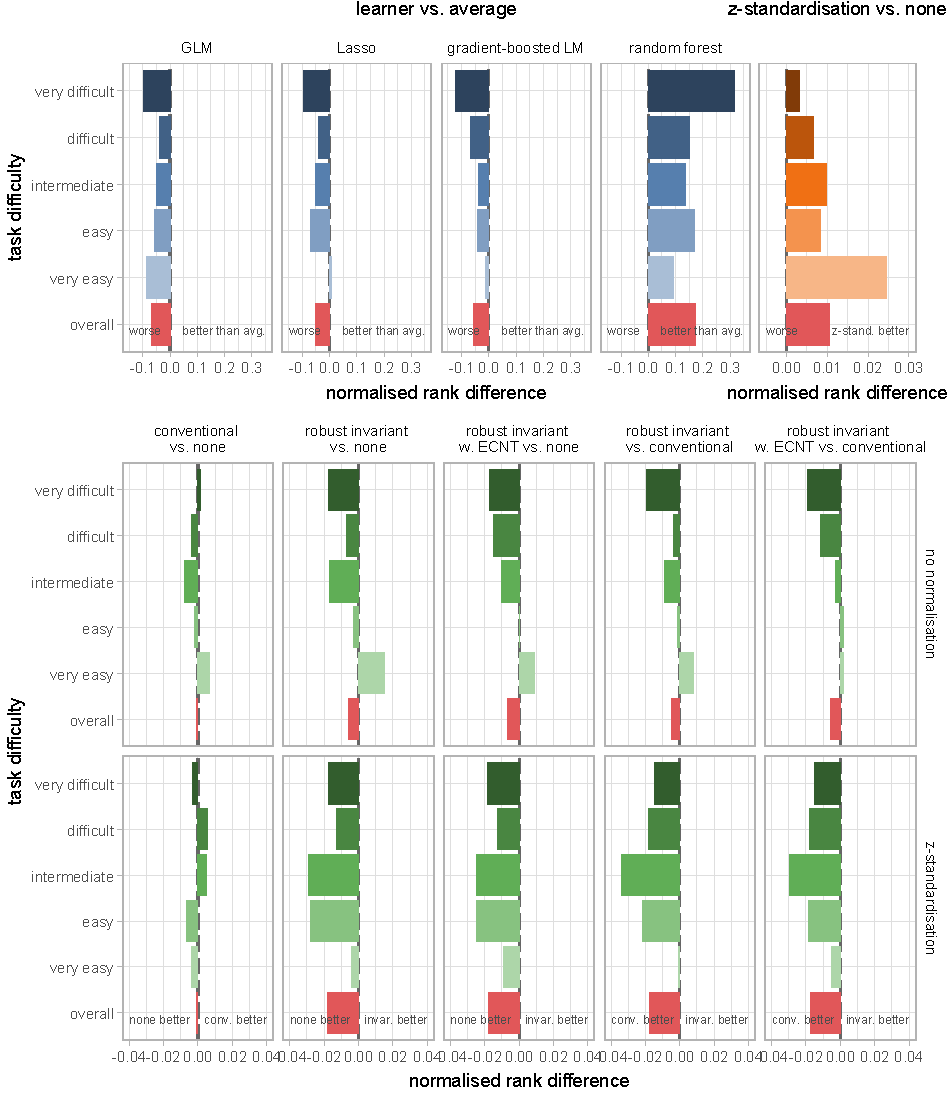
\includegraphics{manuscript_files/figure-latex/marginal-effect-plot-1} 

}

\caption{Estimated marginal effect of learners, normalisation and transformation methods on ranked model performance scores in 18560 machine learning experiments on 232 datasets. The top-left panel shows the marginal effect of learners, i.e. random forests and generalised linear models (GLM). Random forests outperform GLM models for all task difficulties. The top-right panel shows the marginal effect of feature normalisation methods, i.e. no normalisation and z-standardisation. z-standardisation is generally beneficial, but the estimated effect is neglible. The bottom panel shows the marginal effects of different transformation methods, split by learner and normalisation method. There is no consistent behaviour, and estimated effects are neglible. Note that the ranges of the $x$-axes of the three main panels differ. ECNT: empirical central normality test.}\label{fig:marginal-effect-plot}
\end{figure}

\section{Discussion}\label{discussion}

In their work on power transformation, Box and Cox already mention
transformation with a shift parameter, but preferred the version in Eq.
\ref{eqn:box-cox-original} for the theoretical analysis in their paper
(Box and Cox 1964), which subsequently became the convention. Yeo and
Johnson's power transformation lacks a shift parameter altogether (Yeo
and Johnson 2000). We showed that these power transformations are
sensitive to location and scale of data distributions. To mitigate this
issue, we defined location- and scale-invariant variants of the Box-Cox
and Yeo-Johnson transformations. We furthermore assessed methods for
making these transformations robust to outliers, and devised an
empirical test for central normality.

Robust location- and scale-invariant transformations are a suitable
replacement for their conventional counterparts. They demonstrated
robustness against outliers and prevent inaccurate transformations and
potential numerical issues due to location and scale of the distribution
of a feature. This is particularly relevant for automated data
processing, where such issues may go unnoticed. Compared to non-robust
location- and scale-invariant transformations, real-world examples with
outliers showed higher residual errors of transformed features. Robust
transformations seek to minimise residual errors for the central part of
the distribution, instead of the entire distribution, including
outliers. The empirical central normality test indicated that robust
transformations are better able to achieve central normality in the
presence of outliers. However, in a machine learning experiment of 232
real-world datasets that contained at least one numeric feature, we did
not find a meaningful benefit -- nor detriment -- to model performance
for location- and scale-invariant power transformations. One reason may
be that numeric features with large location shifts (\(|\mu| > 1000.0\))
were uncommon. Of the 4886 numeric features in the 232 datasets, 266
(5\%) features in 34 datasets had large location shifts, of which 200
appeared in just 2 datasets. For the latter two datasets, the
transformation method did not show significant difference between groups
(Friedman test; \(p > 0.05\)).

Location- and scale-invariant transformations are realised by
simultaneously optimising three parameters, i.e.~transformation
parameter \(\lambda\), shift parameter \(x_0\) and scale parameter
\(s\). We derived the log-likelihood function to facilitate optimisation
using MLE. Alternatively, standardisation of a numeric variable (e.g.,
through subtracting its median value and division by its interquartile
range) prior to conventional power transformations may achieve a similar
effect in reducing sensitivity to the distribution's location and scale.
While this alternative helps prevent these issues -- provided that
normalisation does not lead to negative values for Box-Cox
transformation -- location- and scale-invariant transformations seem to
provide an overall better transformation to normality (Appendix F).

We assessed several methods for robust power transformation. Methods
that relied on the z-score of the transformed feature or the residual
error yielded worse results than the non-robust method. This is partly
due to the initial choice of threshold parameters. Using different
initial values, closer to the upper limits
(\(\delta_1 = 10.0; \delta_2 = 10.0\)), led to a reduced loss. However,
these values effectively correspond to a non-robust transformation,
where all instances receive the same weight. Underperformance of these
methods could be explained by their use of transformed features for
setting weights. Consequently, the weights change at each iteration in
the MLE optimisation process. This increases local variance in the
log-likelihood function and creates local optima that the optimiser may
not handle well. As a consequence, optimal values for transformation
parameter \(\lambda\) might differ, which increases the presented loss
for optimising threshold parameters. Methods that relied on the
empirical probability did not suffer from this issue, as weights
remained fixed during MLE.

We introduced an empirical test for central normality to assess whether
distributions deviate from normality in a way that might require closer
inspection prior to further processing. The empirical test for central
normality differs from other tests for normality, such as the
Shapiro-Wilk test (Shapiro and Wilk 1965), in that the test statistic is
independent of the number of samples. This makes this test more
practical for assessing central normality for larger sample numbers,
where other tests may detect inconsequential deviations from normality.

This work has the following limitations. Firstly, we did observe several
numerical stability issues for optimisation criteria other than MLE
(Appendix B). These appear in regions where transformation parameters
would lead to very large or small numbers when using conventional power
transformations. For MLE stability issues were not observed. Secondly,
the empirical central normality test is based on simulations instead of
statistical theory, and relies on a somewhat arbitrary definition of the
central portion of a distribution. Thus, while the test may asses
whether data is sufficiently normally distributed for practical
purposes, it should not be used as a strict test for normality.

\section{Conclusion}\label{conclusion}

Compared to their conventional versions, robust location- and
scale-invariant Box-Cox and Yeo-Johnson transformations reduce
sensitivity to outliers and the location and scale of features. An
empirical central normality test can assess the quality of
transformation of features to normal distributions. The combination of
both facilitate the use of power transformations in automated data
analysis workflows.

\section{Data and code availability}\label{data-and-code-availability}

Location- and scale-invariant power transformations were implemented in
the \texttt{power.transform} package for R, which is available from
\href{https://github.com/oncoray/power.transform}{GitHub} and the
\href{https://cran.r-project.org/package=power.transform}{CRAN
repository}. The manuscript was created using R Markdown and is likewise
available from the \texttt{power.transform} GitHub repository. Data and
results for the machine learning experiment are separately available
from \href{https://doi.org/10.5281/zenodo.13736671}{Zenodo}.

\section*{References}\label{references}
\addcontentsline{toc}{section}{References}

\phantomsection\label{refs}
\begin{CSLReferences}{1}{0}
\bibitem[\citeproctext]{ref-Alfons2021-kc}
Alfons, Andreas. 2021. {``{robustHD}: An {R} Package for Robust
Regression with High-Dimensional Data.''} \emph{J. Open Source Softw.} 6
(67): 3786. \url{https://doi.org/10.21105/joss.03786}.

\bibitem[\citeproctext]{ref-Bartlett1947-rx}
Bartlett, M S. 1947. {``The Use of Transformations.''} \emph{Biometrics}
3 (1): 39--52. \url{https://doi.org/10.2307/3001536}.

\bibitem[\citeproctext]{ref-Box1964-mz}
Box, G E P, and D R Cox. 1964. {``An Analysis of Transformations.''}
\emph{J. R. Stat. Soc. Series B Stat. Methodol.} 26 (2): 211--52.
\url{https://doi.org/10.1111/J.2517-6161.1964.TB00553.X}.

\bibitem[\citeproctext]{ref-De-Cock2011-jf}
De Cock, Dean. 2011. {``Ames, Iowa: Alternative to the Boston Housing
Data as an End of Semester Regression Project.''} \emph{J. Stat. Educ.}
19 (3). \url{https://doi.org/10.1080/10691898.2011.11889627}.

\bibitem[\citeproctext]{ref-Gijbels2019-te}
Gijbels, Irène, Rezaul Karim, and Anneleen Verhasselt. 2019. {``Quantile
Estimation in a Generalized Asymmetric Distributional Setting.''} In
\emph{Stochastic Models, Statistics and Their Applications}, 13--40.
Springer International Publishing.
\url{https://doi.org/10.1007/978-3-030-28665-1/_2}.

\bibitem[\citeproctext]{ref-Gorman2014-eo}
Gorman, Kristen B, Tony D Williams, and William R Fraser. 2014.
{``Ecological Sexual Dimorphism and Environmental Variability Within a
Community of Antarctic Penguins (Genus Pygoscelis).''} \emph{PLoS One} 9
(3): e90081. \url{https://doi.org/10.1371/journal.pone.0090081}.

\bibitem[\citeproctext]{ref-Griffin2018-bf}
Griffin, Maryclare. 2018. {``Gnorm: Generalized Normal/Exponential Power
Distribution.''} The R Foundation.
\url{https://doi.org/10.32614/cran.package.gnorm}.

\bibitem[\citeproctext]{ref-Huber1981-su}
Huber, Peter J. 1981. \emph{Robust Statistics}. John Wiley \& Sons.
\url{https://doi.org/10.1002/0471725250}.

\bibitem[\citeproctext]{ref-Kuhn2019-kt}
Kuhn, Max, and Kjell Johnson. 2019. \emph{Feature Engineering and
Selection: A Practical Approach for Predictive Models}. Chapman \&
Hall/CRC Data Science Series. Chapman; Hall/CRC.
\url{https://doi.org/10.1201/9781315108230}.

\bibitem[\citeproctext]{ref-Loprinzi1994-cd}
Loprinzi, C L, J A Laurie, H S Wieand, J E Krook, P J Novotny, J W
Kugler, J Bartel, M Law, M Bateman, and N E Klatt. 1994. {``Prospective
Evaluation of Prognostic Variables from Patient-Completed
Questionnaires. North Central Cancer Treatment Group.''} \emph{J. Clin.
Oncol.} 12 (3): 601--7. \url{https://doi.org/10.1200/JCO.1994.12.3.601}.

\bibitem[\citeproctext]{ref-Nadarajah2005-xe}
Nadarajah, Saralees. 2005. {``A Generalized Normal Distribution.''}
\emph{J. Appl. Stat.} 32 (7): 685--94.
\url{https://doi.org/10.1080/02664760500079464}.

\bibitem[\citeproctext]{ref-Powell2009-zb}
Powell, M J D. 2009. {``The {BOBYQA} Algorithm for Bound Constrained
Optimization Without Derivatives.''} Cambridge NA Report NA2009/06.
University of Cambridge.

\bibitem[\citeproctext]{ref-Raymaekers2024-zf}
Raymaekers, Jakob, and Peter J Rousseeuw. 2024. {``Transforming
Variables to Central Normality.''} \emph{Mach. Learn.} 113 (8):
4953--75. \url{https://doi.org/10.1007/s10994-021-05960-5}.

\bibitem[\citeproctext]{ref-Romano2022-gq}
Romano, Joseph D, Trang T Le, William La Cava, John T Gregg, Daniel J
Goldberg, Praneel Chakraborty, Natasha L Ray, Daniel Himmelstein,
Weixuan Fu, and Jason H Moore. 2022. {``{PMLB} V1.0: An Open-Source
Dataset Collection for Benchmarking Machine Learning Methods.''}
\emph{Bioinformatics} 38 (3): 878--80.
\url{https://doi.org/10.1093/bioinformatics/btab727}.

\bibitem[\citeproctext]{ref-Shapiro1965-zd}
Shapiro, S S, and M B Wilk. 1965. {``An Analysis of Variance Test for
Normality (Complete Samples).''} \emph{Biometrika} 52 (3/4): 591--611.
\url{https://doi.org/10.2307/2333709}.

\bibitem[\citeproctext]{ref-Subbotin1923-qk}
Subbotin, M Th. 1923. {``On the Law of Frequency of Error.''} \emph{Mat.
Sb.} 31 (2): 296--301.

\bibitem[\citeproctext]{ref-Tukey1967-eb}
Tukey, J W. 1967. {``An Introduction to the Calculations of Numerical
Spectrum Analysis.''} In \emph{Advanced Seminar on Spectral Analysis of
Time Series}, edited by B Harris. New York: John Wiley; Sons, Inc.

\bibitem[\citeproctext]{ref-Tukey1957-rt}
Tukey, John W. 1957. {``On the Comparative Anatomy of
Transformations.''} \emph{Ann. Math. Stat.} 28 (3): 602--32.
\url{https://doi.org/10.1214/AOMS/1177706875}.

\bibitem[\citeproctext]{ref-Tukey1977-xm}
---------. 1977. \emph{Exploratory Data Analysis}. Addison-Wesley
Publishing Company.

\bibitem[\citeproctext]{ref-Wright2017-rf}
Wright, Marvin N., and Andreas Ziegler. 2017. {``{ranger}: A Fast
Implementation of Random Forests for High Dimensional Data in {C++} and
{R}.''} \emph{Journal of Statistical Software} 77 (1): 1--17.
\url{https://doi.org/10.18637/jss.v077.i01}.

\bibitem[\citeproctext]{ref-Yeo2000-vw}
Yeo, In‐kwon, and Richard A Johnson. 2000. {``A New Family of Power
Transformations to Improve Normality or Symmetry.''} \emph{Biometrika}
87 (4): 954--59. \url{https://doi.org/10.1093/biomet/87.4.954}.

\bibitem[\citeproctext]{ref-Zwanenburg2021-so}
Zwanenburg, Alex, and Steffen Löck. 2024a. {``Familiar: End-to-End
Automated Machine Learning and Model Evaluation.''} The R Foundation.
\url{https://doi.org/10.32614/cran.package.familiar}.

\bibitem[\citeproctext]{ref-Zwanenburg2024-kq}
---------. 2024b. {``Power.transform: Location and Scale Invariant Power
Transformations.''} The R Foundation.
\url{https://doi.org/10.32614/cran.package.power.transform}.

\end{CSLReferences}

\end{document}
